\documentclass[11pt,xcolor={dvipsnames}]{beamer} % presentation output
% \documentclass[11pt,xcolor={dvipsnames},handout]{beamer} % Beamer printout
% xcolor allows to use many new colors with \usecolortheme

\mode<presentation>{
  \usetheme{Warsaw}
  \usecolortheme[named=OliveGreen]{structure}
  \useoutertheme{shadow}
 	\setbeamercovered{transparent}
	\setbeamercolor{block title example}{fg=white,bg=Blue}
	\setbeamercolor{block body example}{fg=black,bg=Blue!10}
	\setbeamercolor{postit}{fg=black,bg=OliveGreen!20}
	\setbeamercolor{postit2}{fg=yellow,bg=OliveGreen}
}

%% Setting for Beamer printout
\usepackage{pgfpages}
\mode<handout>{
  \usetheme{default}
  \setbeamercolor{background canvas}{bg=Black!5}
  \pgfpagesuselayout{4 on 1}[a4paper,portrait,border shrink=2.5mm]
  % 4 slide in one page
}

\usepackage[italian]{babel}
\usepackage[utf8]{inputenc}
\usepackage{multicol} % Per colonne indice
\usepackage{times}
\usepackage[T1]{fontenc}
\usepackage{graphics}
%\usepackage{numprint}
% with this one \np{1000} becomes 1 000
\usepackage{mathcomp}
%\usepackage{gensymb}
% with this one \numprint[\textcelsius]{20} becomes 20°C
\newcommand{\ud}{\mathop{}\ \mathrm{d}}
% with this one \ud{x} becomes dx
\usepackage{mathtools}
\DeclarePairedDelimiter{\abs}{\lvert}{\rvert}
% to define absolute value (mathtools is required)

\usepackage{listings} % Per la visualizzazione del codice
\usepackage{hyperref}

\usepackage[a-1b]{pdfx} % Per conversione in PDF/A

\hypersetup{
			pdftitle={Interfaccia web per la gestione dei permessi in una piattaforma E-learning per scuole superiori},
			pdfsubject={Interfaccia web per la gestione dei permessi in una piattaforma E-learning per scuole superiori},
			pdfauthor={Taiwo Solomon Olamide},
			pdfkeywords={Ruby, Ruby on Rails, Vue.js, Quasar, PostgreSQL},
			pdfpagemode=FullScreen, % once opened it goes in fullscreen modality
			citecolor=magenta,
			filecolor=green,
			linkcolor=DarkGray,
			urlcolor=Gold
}

\usepackage[absolute,overlay]{textpos}
\setlength{\TPHorizModule}{1mm}
\setlength{\TPVertModule}{1mm}

%%%% A NEW COMMAND TO FIX LOGO POSITION (x,y) in mm
\newcommand{\MyLogo}{%
\begin{textblock}{14}(2.0,80)
%  \pgfuseimage{logo}
 
\includegraphics[height=1.15cm, angle=0]{logo}
\end{textblock}
}
%%%% A NEW COMMAND TO FIX LOGO POSITION (x,y) in mm

%%%%%%%%%%%%%%%%%%%%%%%%%%%%%%%%%%%%%%%%%%%%%%%%%%%%%%%%%%%%%%%%%%%%%%%%%

\title[Interfaccia gestione permessi]{\fontsize{8}{12}\selectfont Interfaccia web per la gestione dei permessi in una piattaforma E-learning per scuole superiori}
\author[Solomon Olamide Taiwo]
{Solomon Olamide Taiwo}
\institute[Università di Ferrara]
{
  %Università degli Studi di Ferrara\\
  Corso di laurea in informatica \\ [0.4cm]
  Relatore\\ Prof. \textbf{Fabrizio Riguzzi}\\ [0.2cm]
  Secondo relatore\\ Dr. Ing. \textbf{Arnaud Nguembang Fadja}\\
  }
\begin{document}
\transduration{1}

%%%%%%%%%%%%%%%%%%%%%%%%%%%%%    TITLE    %%%%%%%%%%%%%%%%%%%%%%%%%%%%%%%
\begin{frame}
	\transdissolve
	\MyLogo
	\begin{center}
		\titlepage
	\end{center}
\end{frame}

%%%%%%%%%%%%%%%%%%%%%%%%%%%% INTRODUZIONE %%%%%%%%%%%%%%%%%%%%%%%%%%%%%%
\section{Introduzione}

\subsection{Introduzione: System Afrik Information Technology}
\begin{frame}{Introduzione: System Afrik Information Technology}
	System Afrik Information Technology (SYAIT) è una realtà ferrarese che si occupa di realizzare soluzioni di alta qualità in ambito web:
	una di queste è una piattaforma E-learning pensata per la gestione di istituti scolastici, per cui durante i mesi di tirocinio
	ho realizzato un modulo per la gestione dei permessi degli utenti utilizzatori del suddetto portale.
\end{frame}

%%%%%%%%%%%%%%%%%%%%%%%%%%%% REQUISITI DEL PROGETTO %%%%%%%%%%%%%%%%%%%%%%%%%%%%%%
\section{Requisiti del progetto}

\subsection{Requisiti funzionali e non funzionali}
\begin{frame}{Requisiti funzionali e non funzionali}
	\transboxin
	%\transblindshorizontal
	% type of transition effect
	\MyLogo
	\begin{columns}[T] % align columns at the top
		\begin{column}{0.5\textwidth}
			\textbf{Requisiti funzionali}
			\begin{itemize}
				\item \textbf{Creazione} dei componenti che visualizzano risorse e azioni;
				\item \textbf{Realizzazione} del layout della pagina principale;
				\item \textbf{Gestione} dei permessi;
				\item \textbf{Accesso} alle funzionalità.
			\end{itemize}
		\end{column}
		\begin{column}{0.5\textwidth}
			\textbf{Requisiti non funzionali}
			\begin{itemize}
				\item \textbf{Prestazioni} adeguate e costanti;
				\item \textbf{Sicurezza}: best practises per realizzazione software sicuro;
				\item \textbf{Usabilità}: applicativo facile da usare;
				\item \textbf{Manutenibilità} del codice.
			\end{itemize}
		\end{column}
	\end{columns}
\end{frame}

\subsection{Diagramma dei casi d'uso}

\begin{frame}{Diagramma dei casi d'uso}
	%\transglitter
	\MyLogo
	\begin{figure}[H]
		\centering
		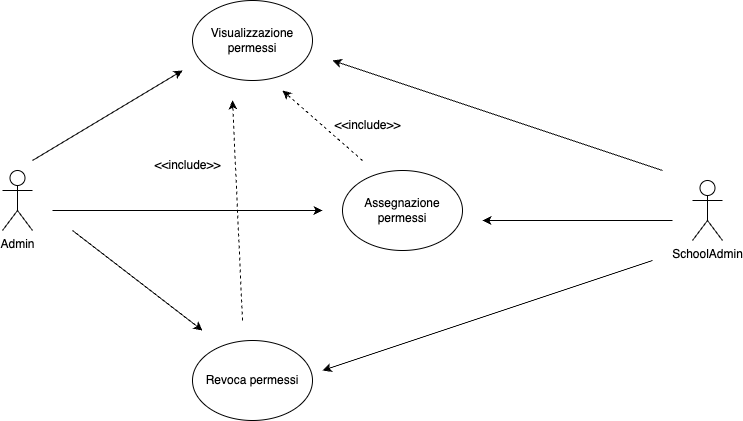
\includegraphics[width=0.9\textwidth]{../images/diagramma-casi-uso-attori.png}
	\end{figure}
\end{frame}

%%%%%%%%%%%%%%%%%%%%%%%%%%%% SECOND SECTION %%%%%%%%%%%%%%%%%%%%%%%%%%%%%
\section{Tecnologie utilizzate}

\subsection{Tecnolologie utilizzate}

\begin{frame}{Tecnologie utilizzate}
	\transboxin
	\MyLogo
	\begin{itemize}
		\item \textbf{Ruby}: linguaggio di programmazione per il backend;
		\item \textbf{Ruby on Rails}: framework per l'utilizzo di Ruby;
		\item \textbf{PostgreSQL}: database per gestione dati;
		\item \textbf{Vue.js}: libreria per JavaScript per la creazione dell'interfaccia utente;
		\item \textbf{Quasar}: framework Vue.js per applicativi desktop e mobile responsivi.
	\end{itemize}
\end{frame}

%%%%%%%%%%%%%%%%%%%%%%%%%%%%%% IMPLEMENTAZIONE DELLA GESTIONE DEI PERMESSI UTENTE %%%%%%%%%%%%%%%%%%%%%%%%%%%%%%%
\section{Implementazione della gestione dei permessi utente}

\subsection{Frontend e backend}

\begin{frame}{Frontend e backend}
	\transboxin
	\MyLogo
	\begin{columns}[T] % align columns at the top
		\begin{column}{0.5\textwidth}
			\textbf{Frontend}
			\begin{enumerate}
				\item \textbf{Design adottato}: utilizzo di mockup
				\item \textbf{Implementazione}: creazione componenti e implementazione in pagina frontend "Permissions"
			\end{enumerate}
		\end{column}
		\begin{column}{0.5\textwidth}
			\textbf{Backend}
			\begin{enumerate}
				\item \textbf{Schema} del database;
				\item \textbf{Inizializzazione} del database;
				\item \textbf{Implementazione}: modelli user e school e controller user.
			\end{enumerate}
		\end{column}
	\end{columns}
\end{frame}

\subsection{Schemi relazionali}

\begin{frame}{Schemi relazionali}
	\transglitter
	\MyLogo
	\begin{figure}
		\centering
		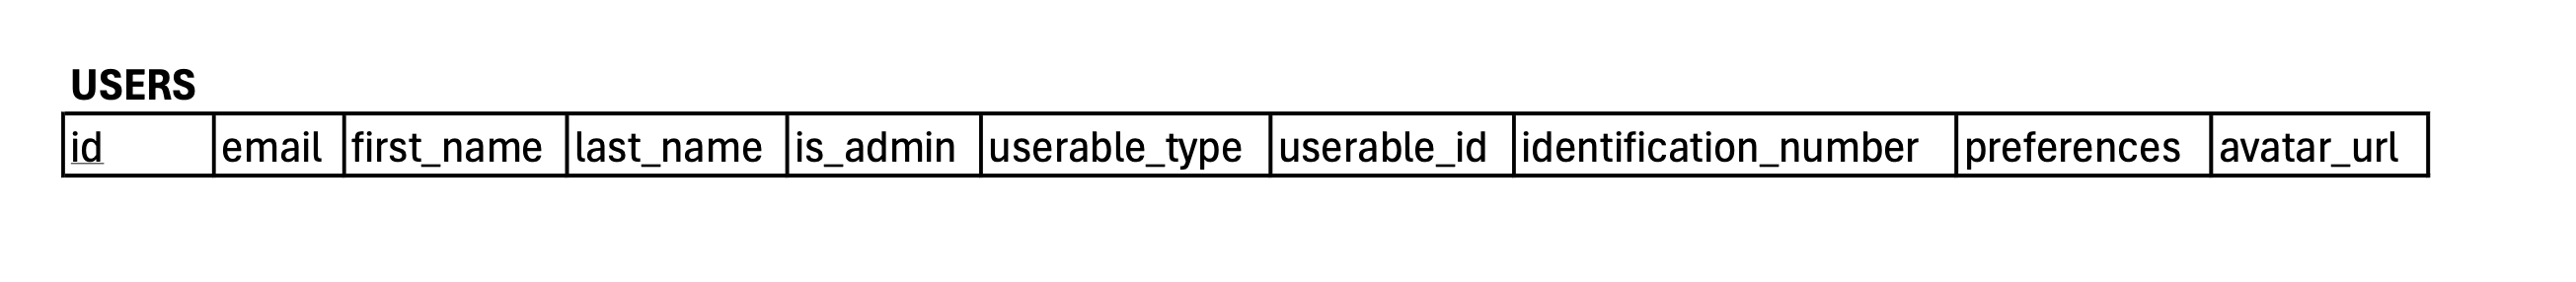
\includegraphics[width=\textwidth]{../images/schema-relazionale-users.png}
		
\includegraphics[width=\textwidth]{../images/schema-relazionale-schools.png}
	\end{figure}
\end{frame}

\subsection{Implementazione frontend finale}

\begin{frame}{Implementazione frontend finale}
	\transglitter
	\MyLogo
	\begin{columns}[T] % align columns at the top
		\begin{column}{0.7\textwidth}
			\begin{figure}
				\centering
				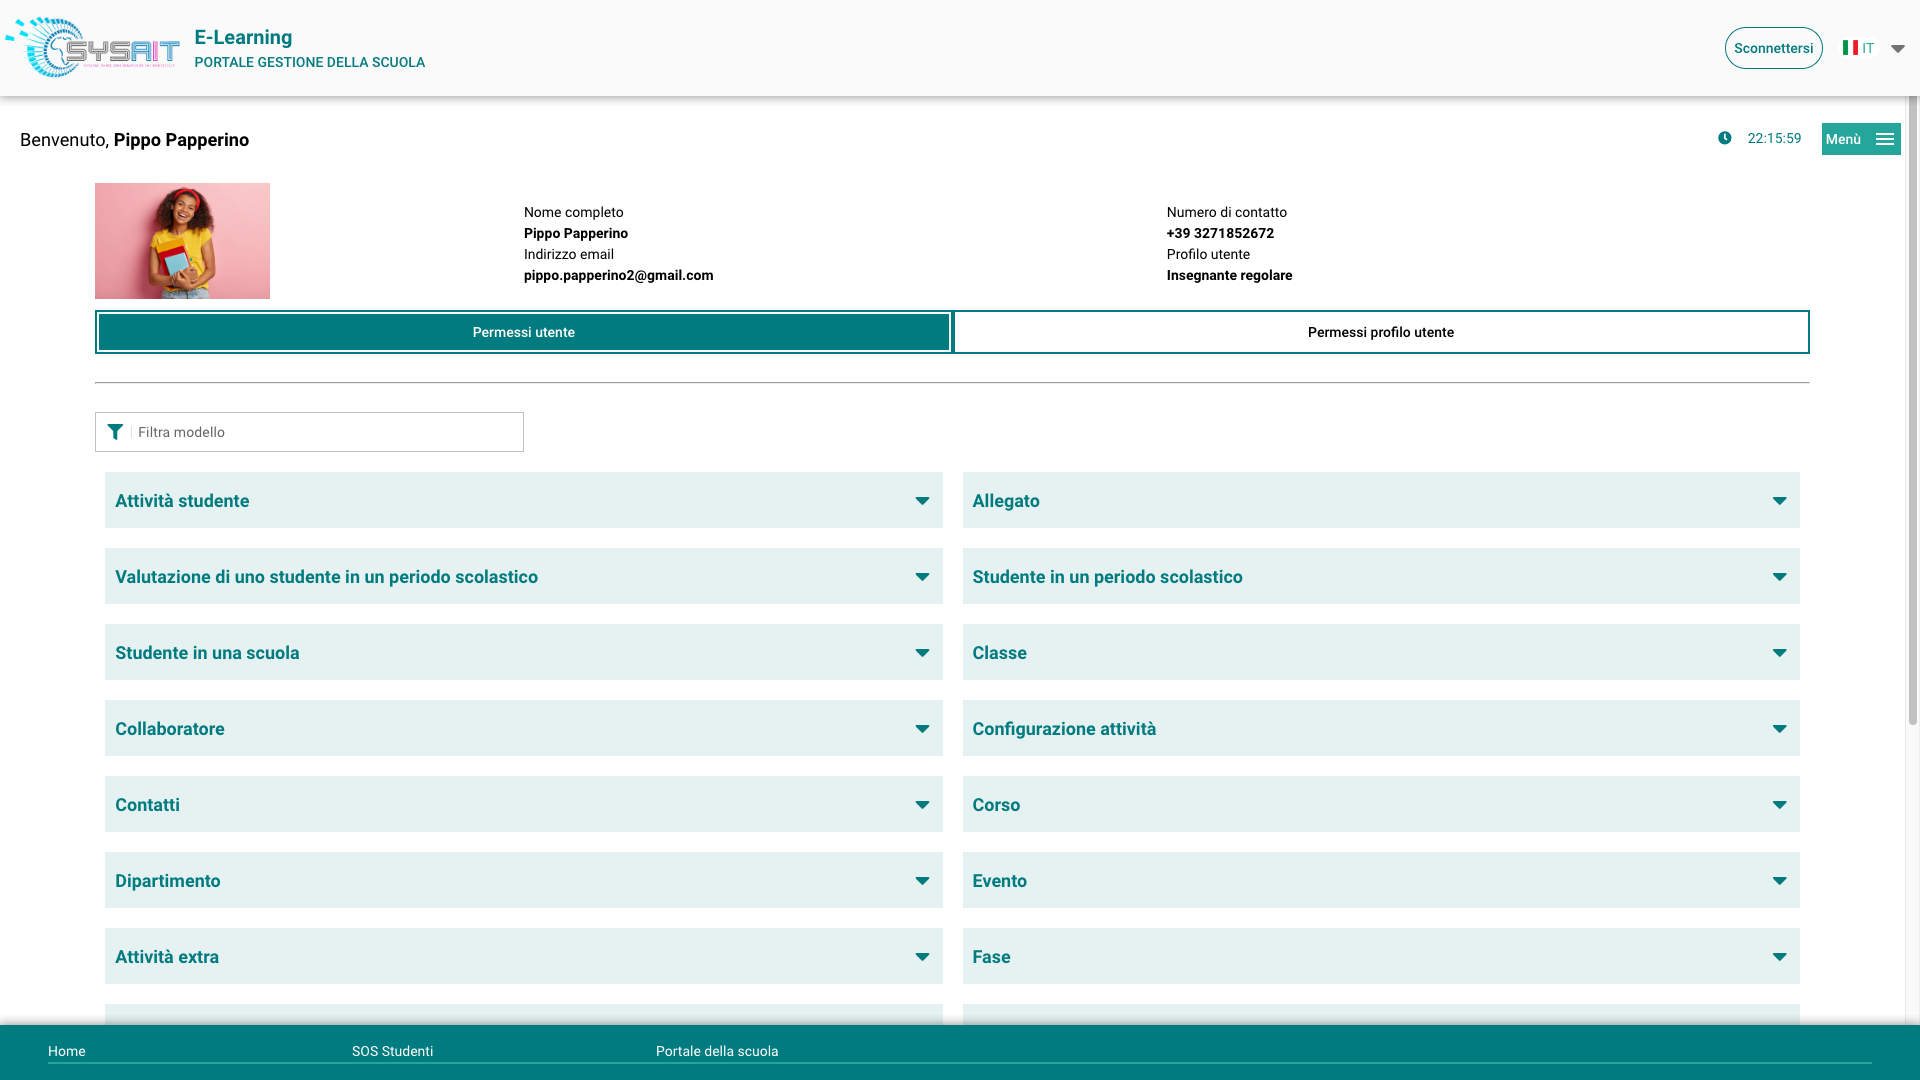
\includegraphics[width=\textwidth]{../images/permission-management-desktop.png}
			\end{figure}
		\end{column}
		\begin{column}{0.2\textwidth}
			\begin{figure}
				\centering
				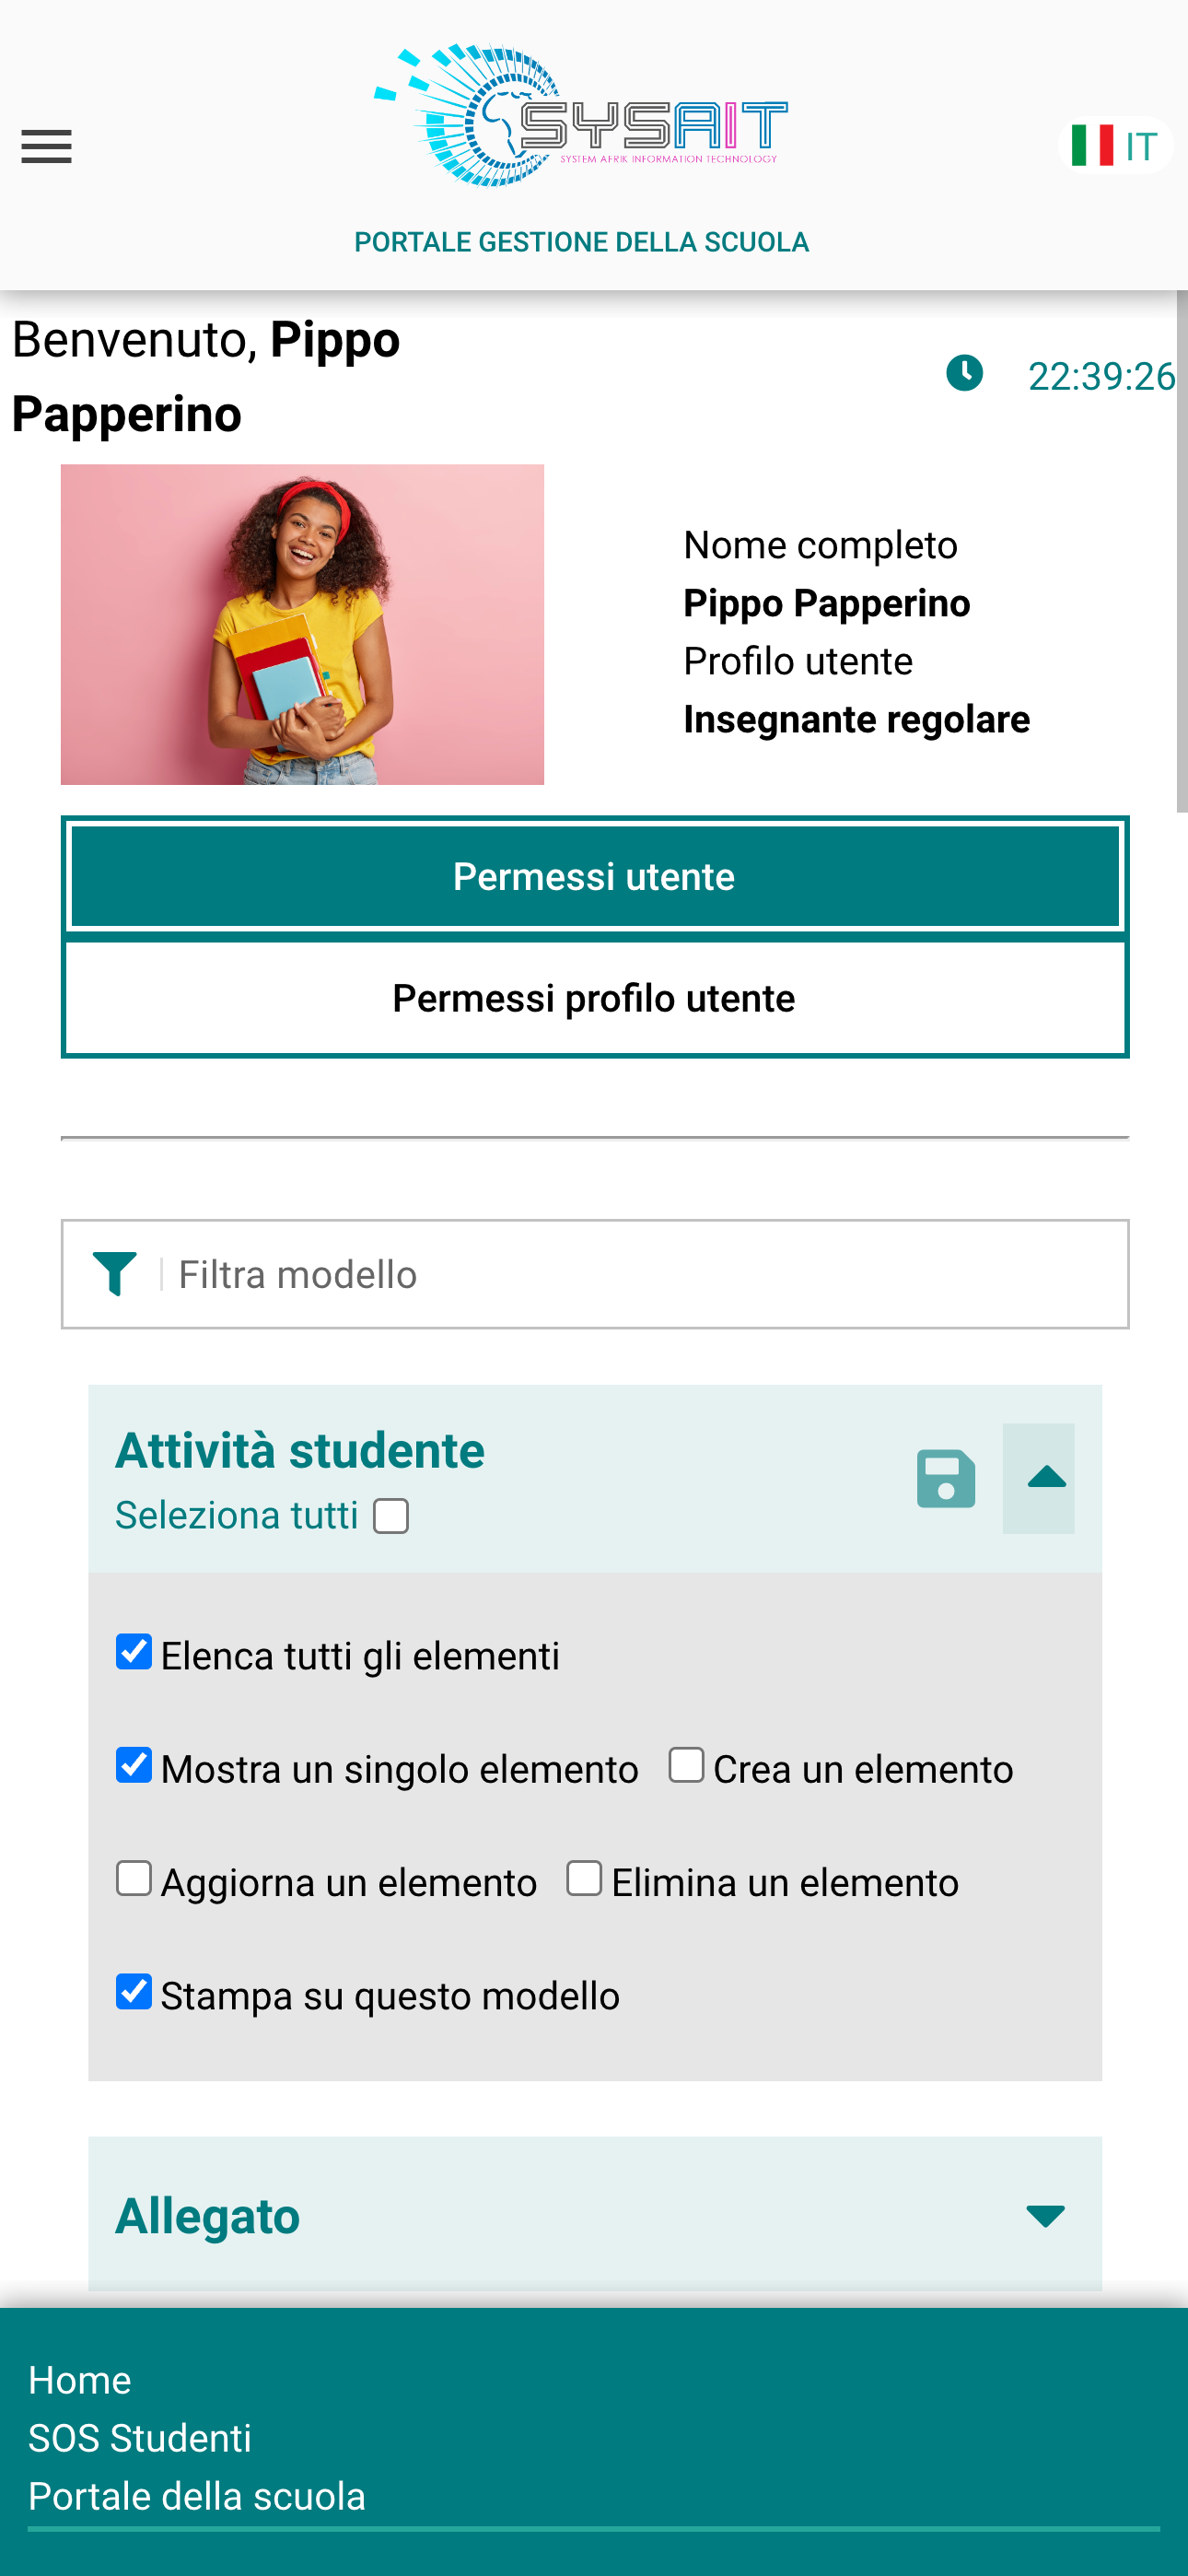
\includegraphics[width=\textwidth]{../images/permission-management-mobile.png}
			\end{figure}
		\end{column}
	\end{columns}
\end{frame}


%%%%%%%%%%%%%%%%%%%%%%%%%%%%%% TEST DELLE FUNZIONALITA' %%%%%%%%%%%%%%%%%%%%%%%%%%%%%%%
\section{Test delle funzionalità}

\subsection{Test del frontend e del backend}

\begin{frame}{Test del frontend e del backend}
	\transboxin
	\MyLogo
	\begin{columns}[T] % align columns at the top
		\begin{column}{0.5\textwidth}
			\textbf{Test del frontend}
			\begin{enumerate}
				\item \textbf{Jest}: framework di testing;
				\item \textbf{Vue Test Utils}: libreria per testing dei componenti Vue.js.
			\end{enumerate}
		\end{column}
		\begin{column}{0.5\textwidth}
			\textbf{Test del backend}
			\begin{enumerate}
				\item \textbf{Insomnia}: tool per verifica del corretto funzionamento delle chiamate
				\item \textbf{Test manuali}
			\end{enumerate}
		\end{column}
	\end{columns}
\end{frame}

%%%%%%%%%%%%%%%%%%%%%%%%%%%%%% CONCLUSIONE %%%%%%%%%%%%%%%%%%%%%%%%%%%%%%%
\section{Conclusione}

\begin{frame}{Conclusione}
	\transboxin
	\MyLogo
	\begin{itemize}
		\item Requisiti funzionali e non funzionali raggiunti;
		\item Interfaccia utente chiara e intuitiva, gestione semplice e immediata dei permessi;
		\item Controllo granulare dei permessi per utenti e profili;
		\item Integrazione con backend Ruby e database PostgreSQL;
		\item Sistema scalabile e manutenibile.
	\end{itemize}
\end{frame}

\end{document}